%% ----------------------------------------------------------------
%% Results.tex
%% ---------------------------------------------------------------- 
\chapter{Model Trainings \& Results} \label{Chapter:Results}

\section{Localised Designs}

Using the simple LSTM design, the number of the LSTM units, the dropout rate, and the batch size are the parameters studied in this section. 
The model has the initial values of 100 LSTM units, a 0.2 dropout rate, and a batch size of 360. 

\subsection{Selecting LSTM Units} \label{Section:units}

Firstly, use 10, 30, 50, 100, 150, 200, and 500 LSTM units to train the model respectively, and record the MSE loss of each epoch. 
The results are plotted in \fref{Figure:simplelstm-unit}. 

\begin{figure}[!htb]
    \centering
    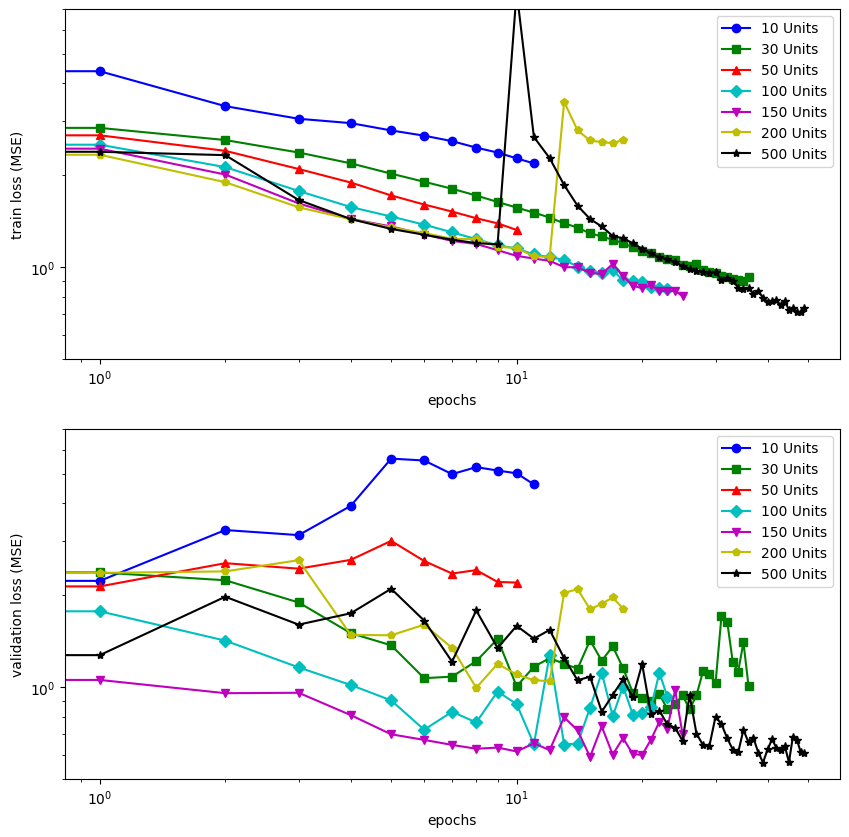
\includegraphics[width=12cm]{simplelstm-unit}
    \caption{MSE losses vs. Epochs of different numbers of LSTM units for both train and validation set}
    \label{Figure:simplelstm-unit}
\end{figure}

In general, the plot shows that the more the LSTM units, the quicker the loss reduces, and the final loss also reduces. 
In theory, larger units result in an LSTM layer with more parameters, which gives the model more capacities to be better at learning complex patterns. 
The LSTM has been designed to effectively capture longer-term dependences, more parameters could also enhance this ability of the model.
Hence, would improve the model's performance. 

Aside from the LSTM layer, an increase in LSTM units also increases the number of connections in the dense layer afterward. 
It not only increases the capability of the LSTM layer but also the dense layer. 

For both the LSTM layer and the dense layer, the time taken for each epoch increases as the number of LSTM units increases. This is straightforward since there are more variables to train each time. 
Increasing time consuming is negligible for first a few numbers of units, but it has a tendency to increase exponentially referring to \fref{Figure:simplelstm-unit-time}. 

\begin{figure}[!htb]
    \centering
    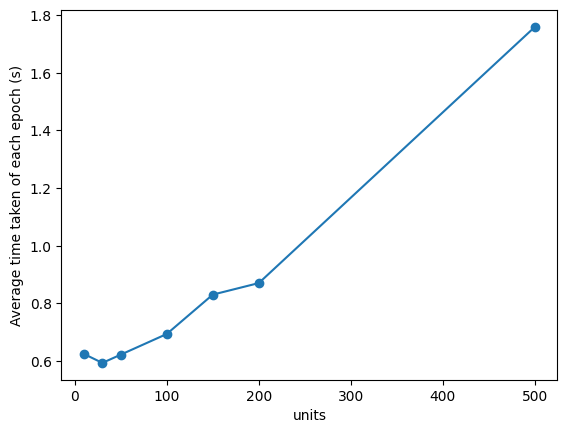
\includegraphics[width=10cm]{simplelstm-unit-time}
    \caption{Average time taken of each epoch vs. number of LSTM units}
    \label{Figure:simplelstm-unit-time}
\end{figure}

Small units like 10, clearly does not have the ability to extract common patterns of the data. The validation loss skyrocketed as the training loss slowly decreased.
The model is overfitting the training data and is not able to adapt unseen data. On the other hand, for larger numbers of units, there is a sudden rise in the training loss. 
It is a sign of the learning rate being too high. The severe fluctuations of the validation loss are another symptom.
A learning rate that is either too high or too low may lead to fluctuations in loss. 

A high learning rate may cause parameter updates too far, which could easily jump over the minimum point, and make it difficult to converge; 
while a low learning rate may cause the convergence speed to be too slow, causing the model to fall into a local minimum. 
This could be optimised by adding a learning rate scheduler in callback functions that update the learning rate dynamically.
The scheduler starts with a larger value of learning rate, 0.001. This learning rate does not change throughout the first 5 epochs.
Starting at the 6$^{th}$ epoch, the learning rate will decrease by a factor of 0.9 every epoch.

\begin{figure}[!htb]
    \centering
    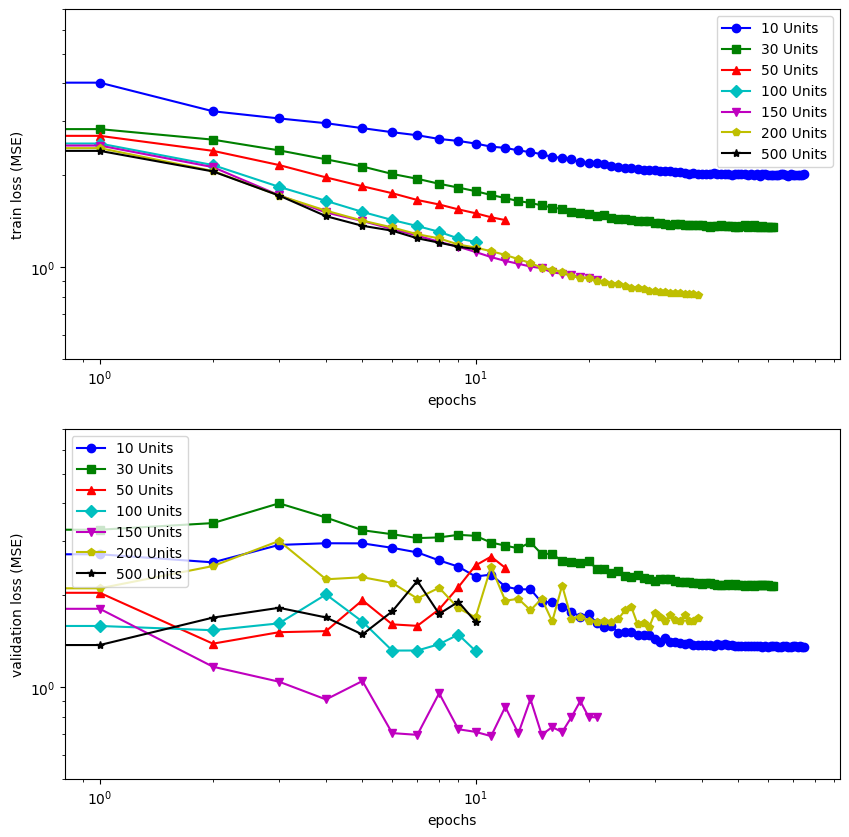
\includegraphics[width=14cm]{simplelstm-unit-lr}
    \caption{MSE losses vs. Epochs of different numbers of LSTM units with the learning rate scheduler}
    \label{Figure:simplelstm-unit-lr}
\end{figure}

After applying the learning rate scheduler, the results are shown in \fref{Figure:simplelstm-unit-lr}. 
This time the curves of both train losses and validation losses are smoother, and there is no sudden rise in training loss anymore. The largest fluctuations are at about 5$^{th}$ to 10$^{th}$ epoch, which is the starting point of the learning rate starts decreasing. 
This tells that the scheduler indeed improves the model as expected. 

For larger numbers of units, the training loss does not improve since 100 LSTM units. Some of them end earlier due to there being no significant drop in validation loss. 
This implies that it is the best performance this architecture given the same input can reach. 
On the other hand, 10, 30, and 50 units underfit the data, the losses are high in both training and validation. 

It has been noticed that each time the curve of the training and validation loss over epochs is different, especially for the validation set. Even the final validation loss is different every time the model. 
This is due to several reasons. Firstly, at the beginning of training, model parameters are initialised randomly. Therefore, even if the same architecture and hyperparameters are used, the initial state of the model is different, which will result in different training outcomes. 
Secondly, in each epoch, the model is updated based on a different batch of data. The sequences in each batch are randomly selected, which will lead to different perturbations for each training. This affects the updated trajectory of the model.
150 units are chosen due to it gives more stable results without having a massive increase in time consumption.

\subsection{Selecting Dropout Rates}

\begin{figure}[!htb]
    \centering
    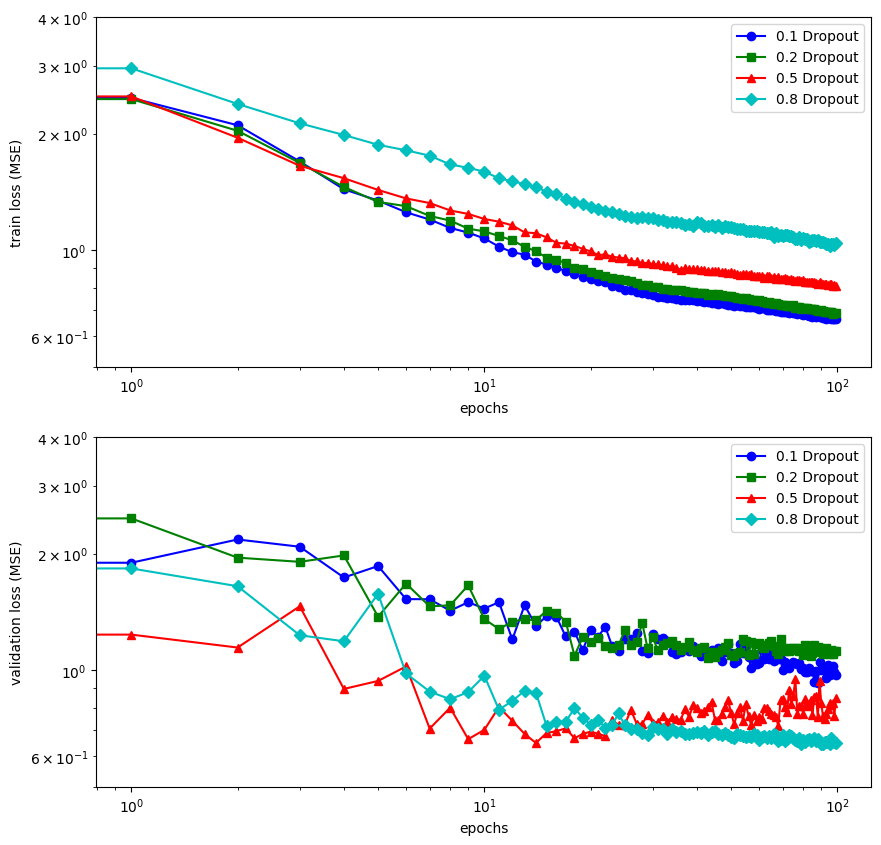
\includegraphics[width=12cm]{simplelstm-dropout}
    \caption{MSE losses vs. Epochs of different dropout rates for both train and validation set}
    \label{Figure:simplelstm-dropout}
\end{figure}

The dropout rates used in this study are 0.1, 0.2, 0.5 and 0.8. Each takes out 10\%, 20\%, 50\%, and 80\% nodes from the network. 
This is designed to prevent overfitting, hence the early stopping strategy is not used to have a better view of the effects caused by the dropout rate.
\fref{Figure:simplelstm-dropout} contains the results of them.

A higher dropout rate can more strongly reduce the overfitting of the model. It discards more nodes in the network, making the network less dependent on specific nodes.
However, a higher dropout rate also reduces the capacity of the model and causes the performance of the training set to decrease. 
On the plot, the lowest dropout rates (0.1 and 0.2) give the lowest training loss, whereas the validation loss of them is higher. 

An appropriate dropout rate is often a trade-off between overfitting and underfitting, thereby improving the overall performance of the model. 
The dropout rate of 0.5 gives roughly the same training and validation loss, it is hence the best choice.

\subsection{Selecting Batch Sizes}

Batch sizes are chosen from 10, 30, 120, 360, 720, and 1440. A large batch size could improve the training speed because each parameter update requires less calculation. 
Using a larger batch size allows the process of gradient descent to parallelise the computation to a greater extent because the sequences could be split across different computation units on the GPU and computed at the same time. 
\fref{Figure:simplelstm-batchsize-time} shows an inverse proportional relationship between the time taken for one epoch and the batch size. 

\begin{figure}[!htb]
    \centering
    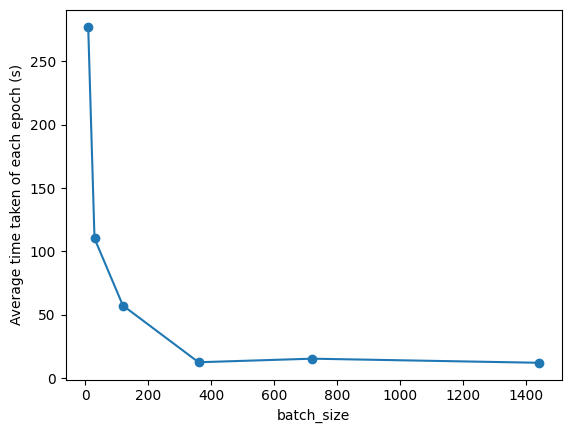
\includegraphics[width=10cm]{simplelstm-batchsize-time}
    \caption{Average time taken of each epoch vs. batch sizes}
    \label{Figure:simplelstm-batchsize-time}
\end{figure}

Different batch sizes may require different learning rates for optimal performance. Typically, larger batch sizes allow for larger learning rates, while smaller batch sizes may require smaller learning rates to avoid exploding or vanishing gradient problems.
To prevent overfitting, the learning rate scheduler explained in \sref{Section:units} and the early stopping strategy are applied. \fref{Figure:simplelstm-batchsize} gives the resulting losses of different batch sizes. 

\begin{figure}[!htb]
    \centering
    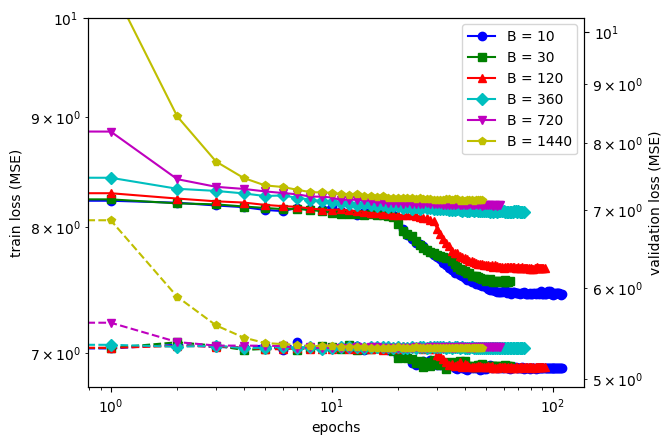
\includegraphics[width=13cm]{simplelstm-batchsize-lr}
    \caption{MSE losses vs. Epochs of different batch sizes for both train and validation set}
    \label{Figure:simplelstm-batchsize}
\end{figure}

In general, the number of iterations required to run an epoch is reduced as the batch size increases. To achieve the same accuracy, more epochs are needed. 
Memory usage is also a key factor when selecting the batch size. Smaller batch sizes can reduce memory consumption because fewer intermediate results need to be stored for each batch. 

A larger batch size can improve the stability of the model and reduce the randomness of parameter updates. 
However, if the batch size is too large, it may cause the model to fall into a local minimum and be difficult to escape.
In the experiment, batch sizes beyond 120 fall into a local minimum, in contrast, small batch sizes have a significant drop during later epochs. 
The drop happened both in train loss and validation loss, showing that this is indeed a better performance rather than overfitting. 

\subsection{Addition of Spatial Features}

By adding the spatial features, with 150 LSTM units, 0.5 dropout rate, 120 batch size, and the implementation of a learning rate scheduler, the training loss of the model drops significantly. 
A plot comparing the previous pure temporal model and the new model is presented in \fref{Figure:spatiallstm}. Both models used the same set of hyperparameters.

\begin{figure}[!htb]
    \centering
    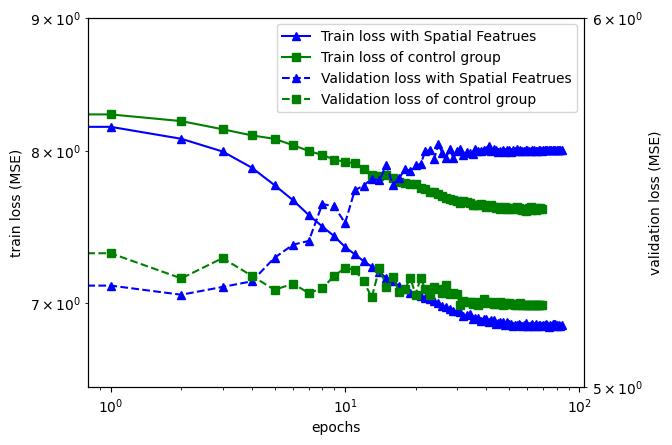
\includegraphics[width=13cm]{spatiallstm}
    \caption{MSE losses vs. Epochs comparing the pure temporal model with the addition of spatial features}
    \label{Figure:spatiallstm}
\end{figure}

The spatial features bring a 10\% reduction in the final train loss, this is significant compared to the difference in previous experiments. 
The validation loss, on the other hand, increases in later epochs, where the pure temporal design does not. 
Any feature change would affect the choice of hyperparameters, hence the process that has been done towards the pure temporal model should be done again. 

\begin{figure}[!htb]
    \centering
    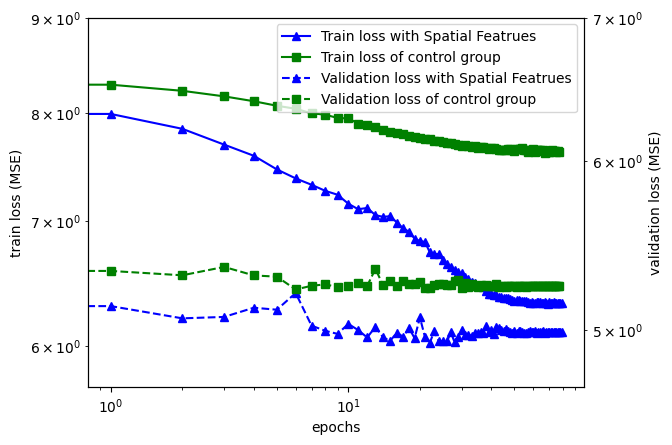
\includegraphics[width=13cm]{spatiallstm-final}
    \caption{MSE losses vs. Epochs comparing the pure temporal model with the addition of spatial features}
    \label{Figure:spatiallstm-final}
\end{figure}

By choosing appropriate hyperparameters, namely 200 LSTM units, 0.2 dropout rate, and 120 batch size, the training loss  reduced 20\% from the control group, without a raise of validation loss. 
The graph has been plotted in \fref{Figure:spatiallstm-final}.
This result shows a close relationship between the current speed of a link and the previous values of its upstreams.
The new features provide a better representation of the data, making the model easier to learn the patterns and the structure. 

Beyond this comparison, the stability of the model is explored. 
8 randomly picked links are trained using the above settings, and the MAPE is used instead of MSE. 
This is because the MAPE focuses on the relative difference, making the loss comparable between different links. 
\tref{Table:spatiallstm-links} shows the results. 

\begin{table}[!htb]
    \centering
    \begin{tabular}{c|cccccccc}
    \toprule
    ID & 118 & 36 & 47 & 88 & 114 & 70 & 21 & 74 \\
    \midrule
    Train MAPE & 72.45 & 78.88 & 78.15 & 78.88 & 79.55 & 78.39 & 77.61 & 70.22 \\
    Val MAPE & 76.25 & 79.05 & 78.73 & 79.50 & 79.83 & 79.83 & 78.76 & 80.98 \\
    \bottomrule
    \end{tabular}
    \caption{Trian and validation MAPE loss of 8 randomly picked links}
    \label{Table:spatiallstm-links}
\end{table}

The result does show a good stability of the model. The train loss varies not much in the range between 70 to 80. 
The difference is caused by the number of upstreams the link has. There are four features representing the speed in the upstreams. 
For the links only contain one or even no upstreams, such features are wasted. 
The above discussion has proven that such features have a positive impact on its performance, different links may benefit differently from these features. 

Also, based on the analysis of data in \sref{Section:TemporalData}, each link seems to have a unique distribution of data. 
Even if the data is similar, the model is more sensitive to certain features, and the importance of these features may differ in different links. 

\section{Globalised Designs}

\subsection{ST-LSTM}

Different from the localised designs, the ST-LSTM model minimise the loss by only using two epochs. Every time the loss reaches its minimum at the second epoch. 
It can be a good sign that the model has adapted well to the training set. The characteristics of data are learned in a short training period. 
Conversely, it can also be a sign of underfitting, that the model only captures the simple patterns of the data, and cannot further improve.

Instead of giving the whole training set and validation set to the model, those two sets are given by sequence generators. 
A total of three generators responsible for the training, validation, and test set were used, which means the data were separated before the sequences formed. 
This allows the training and validation set to separate completely. 

By tuning the batch size, the training and test loss stays the same, however, the validation loss increases as the batch size increases. 
The results are gathered in \tref{Table:stlstm-batchsize}. The validation loss increase is as expected since a larger batch size introduces more noise and makes the generalisation ability of the model decrease. 
The training loss, on the other hand, seems to fall into a local minimum and cannot escape. It is a sign of underfitting. 

\begin{table}[!htb]
    \centering
    \begin{tabular}{c|ccccc}
    \toprule
    B & 120 & 360 & 720 & 1440 & 5040 \\
    \midrule
    Train MSE & 1.8701e-04 & 1.8701e-04 & 1.8701e-04 & 1.8701e-04 & 1.8701e-04 \\
    Val MSE & 4.7873e-05 & 1.1068e-04 & 2.22036e-04 & 3.2226e-04 & 3.7096e-04 \\
    Test MSE & 2.2528e-04 & 2.2528e-04 & 2.2528e-04 & 2.2528e-04 & 2.2528e-04 \\
    \bottomrule
    \end{tabular}
    \caption{Minimum MSE losses vs. Batch sizes of ST-LSTM model}
    \label{Table:stlstm-batchsize}
\end{table}

This model can be considered as unsuccessful, the structure of the model designed is not suitable for the problem. 
To improve its performance, it is reasonable to change the architecture. 

\subsection{GCN-LSTM}

\begin{figure}[!htb]
    \centering
    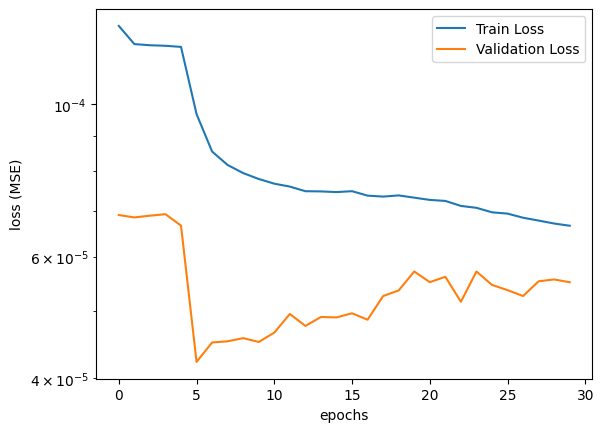
\includegraphics[width=12cm]{gcnlstm_loss}
    \caption{MSE losses vs. Epochs of GCN-LSTM model}
    \label{Figure:gcnlstm_loss}
\end{figure}

The model easily overcomes the local minimum point and trains further down the gradient. 
The performance has been improved by using the GCN layer. The path of the losses over epochs is shown in \fref{Figure:gcnlstm_loss}.
